% Typeset by:
%  Will Crawford (wacrawfo@ucsc.edu)

% TODO:
% Most occurrences of ``the algorithm'' should be replaced by ``the scheduler.'' DO NOT do a global find/replace.
% Check on instances of ``he.'' They should probably be changed to ``he/she.''

%%%

% Development Process: Explain the phases of Unified Process.
% Rewrite Scenario 4 and possibly provide a mockup.
% - System should review integrity of schedules, not the administrator. 
% New diagrams around line 200?
% Replace symbols in the diagrams of Requirements: Specification
% Consider removing the old diagrams
% Do we need to mention the fitness function in 4.3: The Algorithm?


%%%%%%%%%%%%%%%%%%%%%%%%%%%%%%%%%%%%%%%%%%%%%%%%%%%%%%%%%%%%%%%%%%%


\documentclass[12pt]{article}
\usepackage{amsmath}
\usepackage{graphicx}
\usepackage{fancyhdr}
\pagestyle{fancy}
\fancyfoot{}
\rfoot{\thepage}

\graphicspath{{./img/}}
\setlength{\parskip}{0.15in}

\title{S.C.O.R.E Report for\\ MyCourses \\ A Course Scheduling System \\ UCSC Team}
\author{Ben Ross \texttt{(bpross@ucsc.edu)} \\
	\and Erik Steggall \texttt{(esteggal@ucsc.edu)}\\
	\and Justin Lazaro \texttt{(jlazaro@ucsc.edu)}\\
	\and Sabba Petri \texttt{(spetri@ucsc.edu)}\\
	\and Will Crawford \texttt{(wacrawfo@ucsc.edu)}}
\date{}

\begin{document}

\maketitle
\pagebreak
\tableofcontents
\pagebreak

\section{Executive Summary}
The MyCourses Scheduler is an end-to-end scheduling system that automates and reduces the manual labor of scheduling university courses. We seek to provide universities an easy-to-use and automated service that can help reduce staff costs, reduce implementation costs and decrease the complications and time involved in organizing an entire schedule.


The team started in mid-September by a group of 5 engineering students taking a ``Software Methodology'' course. We chose to do a course scheduling system as our class project because, like many other students and faculty, we felt that the problem was an interesting one, and that we would learn a lot by writing a system to solve it.

The members of our team are Justin Lazaro, Will Crawford, Ben Ross, Erik Steggall, and Sabba Petri. Our team members have held a variety of roles in the technology industry such as IT, QA, Marketing and System Administration at top technology firms including Hewlett Packard, Riverbed Technologies, and Yahoo!. 


We believe that our solution can provide value to universities and ease the frustrations of faculty, students, and staff. In addition to a course scheduling system, we plan on expanding our product line to include an employee scheduling system and offer that as a Software-as-a-Service to businesses nationwide. 

% Review again for tense
\section{Development Process} % Will
\indent This instance of the MyCourses course scheduling system was created as part of a class instructed by Professor Linda Werner here at UCSC.

Participation in this class required us to approach design very seriously before we started coding. This was a new approach to us; most of us were tempted to go directly for some sort of rapid prototype.

After gathering the requirements from the SCORE project description, we analyzed them, immediately discovering that scheduling classes would probably be NP-hard, meaning that there would be no way to find an optimal solution in polynomial time. In other words, it looked like a problem with no canonical ``best answer.'' Much of our time in this phase was spent shopping around for an appropriately similar problem that we could model our actual problem on. We eventually found a solution to the problem in the form of a freely available course scheduling algorithm written by a graduate student in C++ which we converted into Python.

We started out our project using the Unified Process, an iterative and incremental software development process, to plan our project. The Unified Process is composed of four phases: inception, elaboration, construction and transition. 

% Explain the phases here.

Because of our lack of familiarity with the technology, we planned on using for our project - Django, our Python web framework, in particular - much of our inception and elaboration phases were spent learning about the functionality and capabilities of these technologies so that we would be more able to generate realistic design documents for our project.

Since this project was being done as part of a class, our instructor required several deliverables from us apart from the requirements of the SCORE project - primarily presentations and the delivery of documents - as part of a modified Unified Process for development. 

For our first deliverable, part of our inception phase, we wrote out scenarios for the use of our product. We included a scenario for each of the user categories that would be using our product. Our program administrator scenario described how the program administrator would initially set up the database in order to run the algorithm. The scenario for the program manager shows how the program manager should be able to inspect the courses that the administrator picked, and select the courses and lecturers for the upcoming quarter. The scenario for the lecturer shows how the lecturer should be able to specify their own individual constraints, such as the courses that they wish to teach, and the days and times that they are available. The scenario for the student shows how a student should be able to select a course for their upcoming quarter. We also included a scenario in which the program administrator can receive the master schedule from each individual program manager and is then able to set up and run the algorithm.

Our second deliverable provided an overview of our requirements, also part of our inception phase. In this deliverable we provided a broad overview of our system and its functionality. It was broken into functionality, performance, usability, constraints, and our wish list. The functionality provides a description of what our system does, we included information on the algorithm, a breakdown of our database, the different sections of our user interface, and the specifications of our server.

Our third deliverable was an overall summary of our project, part of our elaboration phase. We provided a high level architecture that showed the break down of our system into user interface, Django, and the algorithm. We went into detail on how we planned to build our project and reasons for building it the way we did. We also included interaction diagrams, in which we elaborated on the scenarios we selected. 

Our fourth deliverable was a user manual for our project, part of our construction phase. This deliverable was primarily a tutorial for each user role showing how they will use our final product. It had a step-by-step process for setting up accounts and performing the necessary tasks for each role. Our user manual also includes a system overview so that it is more clear for the user reading it.

Our final deliverable was an acceptance test for our project. This deliverable was a working prototype designed to exhibit the same qualities that our final product will have. It demonstrated most of  our project's functionality, though it was far from feature-complete.

\section{Requirements: Problem Statement} % Justin
At many Universities, scheduling courses becomes a difficult task for many registrars office. The task of manually scheduling hundreds of courses with limited classroom space, limited professor availability, and limited time is an extremely difficult and long task. With our Scheduling system, we developed an end-to-end course management system that simplifies and automates the quarterly (or semesterly) scheduling of courses for universities. Our system will offer features including automated organization of these courses and management of classes \& professors. It will also allow students to sign up for classes. With this system, we hope that it will reduce the difficulty and time of managing and scheduling courses. 

Our system will have four primary user groups: Program Managers, Program Administrators, lecturers, and students. The Program Administrator will be responsible for managing and populating of the system with courses, classrooms and time slots. Program Administrators will also be responsible for running the Scheduler. The Program Managers will select courses to offer in the given quarter and provide additional information such as class size and class location. The lecturers (or professors) will be able to define their course preferences and also their time slots they prefer.  The students will be able to sign up for the courses scheduled by the system.

Our project includes the ability to define the constraints of courses, classrooms and professors. By offering this amount of flexibility, we can reduce the overhead cost and time necessary to schedule courses. Below we outline a common scenario for each category of users. 


\subsection{Scenario}
At the beginning of the inception phase, we generated and utilized scenarios to help us understand the expected user interaction with our system. We developed several scenarios that relate to each user groups� interaction with our scheduling system. The following is an example of a Program Administrator�s and Program Manager�s interaction with the Scheduling system and how the database is initially populated and managed after it is populated.

\begin{enumerate}
\item	The Program Administrator signs in to the browser-based MyCourses system by supplying their credentials to the website.
\item	Once logged in, the Program Administrator is presented with a panel illustrating their privileges - there will be links to pages that let the admin modify the database, add users, etc.
\item	The Program Administrator can click on the database modification link, and will subsequently be presented with its contents in a tabular format.
\item	Choosing to import data, the Program Administrator will need to provide the following: 
	\begin{enumerate}
	\item	A list of all classrooms and buildings available, including...
		\begin{enumerate}	
		\item Room capacity.
		\item Subject preference. (e.g. Social Sciences belong in the Sociology building)
		\end{enumerate}
	\item	List of all instruction time slots. (e.g. Can classes be taught on Saturday? When are normal instruction hours?)
	\item	List of courses offered for every subject. 
	\end{enumerate}
\item	The Program Administrator can also manually enter information (e.g. Baskin Engineering $\to$ Room 156 ) or modify imported information. This can be done by clicking on the appropriate element, modifying the appropriate fields, and submitting the changes.
\item	Once the information has been imported and reviewed, each Program Manager can determine which courses will be offering in the upcoming quarter.
\item The Program Manager sign in to the browser-based MyCourses system by supplying their credentials to the website.
\item The Program Manager sees a message that notifies them that the system has been populated by the Program Administrator for a new quarter and opens a list of all the courses in their department.
	\begin{enumerate}
	\item The Program Manager will be able to select which courses will be offered for this particular quarter.
	\item The Program Manager will also be able to specify which instructor will teach each course.
	\end{enumerate}
\item After each Program Manager has completed this task and their work has been saved, the Program Administrator will be notified via e-mail.
\item The Program Administrator can then log in. He or she can review the entire list of courses if he or she chooses. The Program Administrator is also able to run the scheduler at this point, which will algorithmically determine when courses will be taught. The system will attempt to provide a best fit and present that to Program Administrator for review, modification, and/or acceptance.
\end{enumerate}

\section{Requirements: Specification} % Sabba
This section is designed to provide an overview of the MyCourses Scheduler based on the requirements above. Within this section, one will understand the power behind the technology used for this system: the web server technology and the algorithm used to schedule the classes. To begin, the web server for the MyCourses Scheduler system is irrelevant so long as it works with Django, the web framework we chose. The strictly because of its ability to ease the creation of database-driven websites. It provides an abstracted framework for dynamic websites that is easy to learn and easy to integrate. The available components also will help us throughout this design process, such as the templating system interfacing with the user interface. Django is written in Python, which is the language of choice for this project, as well as the language of our algorithm.

When deciding upon an algorithm, we needed to decide whether to go with a constraint-based solver, or to design an algorithm in-house to fulfill out needs. Because the scheduling problem is an NP-Hard problem, a constraint-based solver would facilitate the implementation of the scheduler. However, learning to use a constraint-based solver would require more time to learn. On the other side to this decision, designing an algorithm in-house would provide full control of the algorithm in how we decide to integrate it with the web server framework.

Figure three displays the class diagram of our project., the class diagram depicts an overall outlook of our in-house algorithm, of which will be the heart and engine of our Scheduling system. This class diagram shows the relationship between the configuration Python file with the different database attributes, such as professor, course, room, schedule, and course class. The configuration class is the primary driver that weaves all the user groups and database attributes together to function as a single entity.  

% See http://en.wikibooks.org/wiki/LaTeX/Importing_Graphics#Images_as_Figures
%\begin{figure}[!h]
%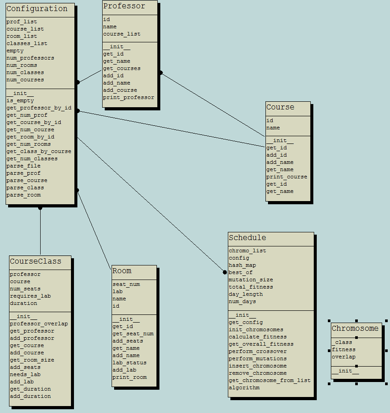
\includegraphics{classDiagram.png}
%\caption{Class Diagram of Algorithm}
%\end{figure}

% Perhaps there could be a diagram for the below.
The interaction diagrams below contain interactions of each user: student, lecturer, program manager, and program administrator. Each diagram details a pictorial representation of the user: interaction with the system, such as the website, the Django engine, the database that handled, or the algorithm itself.  In all these diagrams, the portal, or front-end website, is an input/output object wherein users will input items and receive output from Django. From behind the front-end website, Django serves as a control object that handles all aspects of user, algorithm, and database interactions. The database itself is an entity that stores information from user input processed by Django, and it also provides output to the user. Lastly, the algorithm is a control entity that manipulates the database courses, but all functionality of the algorithm remains hidden from the entire system. 
%\pagebreak

%\begin{figure}[!h]
%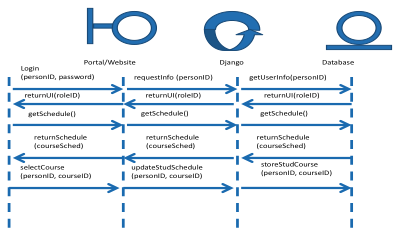
\includegraphics{studentID.png}
%\caption{Student interaction diagram}
%\end{figure}
%\pagebreak
\begin{enumerate}

\item The student will login with their ID and password on the portal. Django will read the ID and password and match it with the database. 
\item Once the database confirms user, the database will return the correct UI for the student.
\item The student will want to get the schedule of classes to sign up for and makes a request to Django and the database to display the available courses. By making a request, this is done invisible to the user and the user will simply click on the courses tab. It will open automatically for the user. 
\item The student can now select courses and store them into their profile on the database. 
\end{enumerate}

%\begin{figure}[!h]
%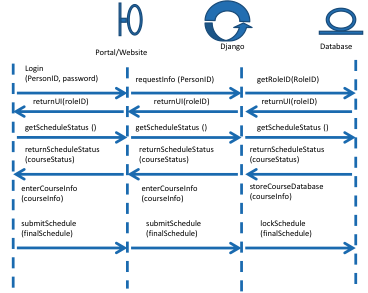
\includegraphics{programAdminID.png}
%\caption{Program Admin enters courses interaction diagram}
%\end{figure}

\begin{enumerate}
\item The program administrator will login with their ID and password on the portal. Django will read the ID and password and match it with the database. 
\item Once the database confirms user, the database will return the correct UI for the program administrator.
\item The program administrator will want to know the status of the schedule, to see if it is finished or not, and will make a request to both Django and the database to find out the status. 
\item The database will return the status. 
\item The program administrator will begin filling out course information through a courseInfo object that will contain various data about a given course.
\item When the program administrator feels done, they can choose to submit the course and lock the course in the database. 
\end{enumerate}

%\begin{figure}[!h]
%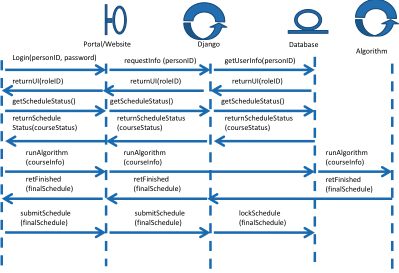
\includegraphics{programAdminID2.png}
%\caption{Program Administrator runs algorithm interaction diagram}
%\end{figure}

\begin{enumerate}
\item The program administrator will login with their ID and password on the portal. Django will read the ID and password and match it with the database. 
\item Once the database confirms user, the database will return the correct UI for the program administrator.
\item The program administrator will want to know the status of the schedule, to see if it is finished or not, and will make a request to both Django and the database to find out the status. 
\item The database will return the status to see if the program manager has completed the schedule. 
\item If the schedule is complete, the program administrator will run the algorithm that will be passed through Django and straight into the algorithm engine.
\item When the engine has completed, it will return a message that it is complete to the HTML website. 
\item Once the program administrator reviews the schedule, the program administrator can submit and lock the schedule and provide it to students
\end{enumerate}

%\begin{figure}[!h]
%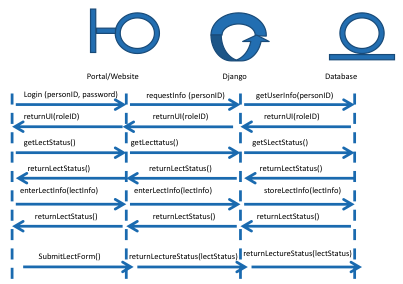
\includegraphics{lecturerID.png}
%\caption{Lecturer interaction diagram}
%\end{figure}

\begin{enumerate}
\item The lecturer will login with their ID and password on the portal. Django will read the ID and password, and match it with the database. 
\item Once the database confirms user, the database will return the correct UI for the lecturer.
\item The lecturer will want to find out the constraint form has been completed. Upon logging in, Django will send a message on the status of his constraint form, based upon a status in the database.
\item The lecturer will fill out the constraint form and store it in the database.
\item Upon storing it in the database, the lecture status will be updated and confirmed. 
\item The lecturer can now formally submit his constraints form to the database. 
\end{enumerate}

%\begin{figure}[!h]
%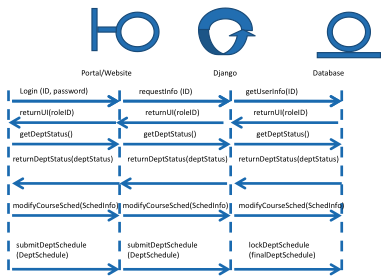
\includegraphics{programManagerID.png}
%\caption{Program Manager interaction diagram}
%\end{figure}

\begin{enumerate}
\item The program manager will login with their ID and password on the portal. Django will read the ID and password and match it with the database. 
\item Once the database confirms user, the database will return the correct UI for the program manager.
\item Upon logging in, Django will automatically send a request to find out the department status of the courses. 
\item If the status is not yet been completed, it will send a message to the program manager.
\item The program manager can modify the courses that was made available from the program administrator and placed in the database. 
\item Upon modifying the courses and the course info, the program manager can confirm and submit the finalized course. 
\end{enumerate}


\section{Architectural Design} % Erik
Our architecture is broken into three main categories:
\begin{enumerate}
\item User interface or UI (The front end)
\item Django (The back end)
\item The Scheduler (The engine)
\end{enumerate}

\subsection{The User Interface}
There are four different user interfaces, each is assigned to one of the four roles that a user could be: Program administrator, program manager, lecturer, student. The students UI is the most complex and offers the most customization.

The program administrator's user interface is fairly simple, they are given fields such as courses, rooms, and professors to fill out, once they fill out the fields to the proper specifications for the quarter then they have an option to run the Scheduler. The Scheduler will run, and then post the results to the program manager.

The program manager's interface will display all of the courses and lecturers for their department. The program manager will have the option of selecting the lecturers and courses that they want to be active for the quarter.

The lecturer will have an interface that will hold the courses that they can teach and the current courses that they are teaching. 
The student will have a customizable interface which will hold their past, present and future schedules. It will also have other widgets that they will be able to add to their profile.
\subsection{Django}
Django connects the user interface, the database and the Scheduler. Django manages the user interface by handling the user requests and providing the appropriate response. In the case of the Scheduler it takes the request from the program administrator to run the Scheduler and creates a request object and sends it through multiple middlewares (Python functions). Django then checks the URLs and determines which function it must send the request object. The function in this case is the Scheduler, which takes the information stored in the program administrators database and runs. The output of the Scheduler is placed into a second database and the request object is sent back up through the middleware in the reverse order of the way it came in. The second database is then displayed to the program administrator.

\subsection{The Scheduler}
The algorithm we use is a modified genetic algorithm, which mimics the process of natural selection in order to find the solution to our scheduling problem. The algorithm represents the variables as chromosomes. A full set of chromosomes make up a parent, each parent is given a fitness value according to how well they fit into the schedule. Fitness is higher for matches that fit into empty classrooms, have the appropriate number of seats, or if the class has a lab in it. The parents make up a population, the algorithm takes 'n' number of parents from the population and does a crossover on pairs of the selected parents to create 'n' new chromosomes. The algorithm replaces 'n' chromosomes from the existing population with the new chromosomes that were created by the crossover, however it does not replace the chromosomes with the best fitness. After the crossover is performed, mutations take place. A random number is generated, which represents the mutation size. While the size has not been reached, classes are moved at random to a random room. Classes with the best fitness are ignored. The algorithm repeats this process until it reaches a fitness of one, in which has it has found an optimum solution. The algorithm pulls information from the database, and enters it into four different list: a professor list, a course list, a room list and a classes list. It then outputs into a second database which is then displayed to the user interface.

\section{Project Plan} % Justin

The project plan will describe the date and deliverables of our development process. The SCORE project followed a software methodology course and many of the deliverables are similar to those in the SCORE requirements. 

Instruction and classes began on September 23, 2010 and continued for 10 weeks until the end of the quarter. Further development of our scheduling system will continue on to the winter quarter starting January 4, 2011 through March 18, 2011. 

\subsection*{Week 1: Initial Presentation}

For the first week, we had to gather in groups of 5 to form teams for our project and give an initial presentation on a brief overview of our project. 

We covered the following items:
\begin{itemize}
\item Team name
\item Team members
\item User experience
\item Core functionality
\item Wish list
\item Possible project risks
\end{itemize}

\subsection*{Week 2: Requirements - Scenarios}

During this week, our team designed several user scenarios related to our project. The scenarios will be a significant part of our requirement document and will be important in defining various aspects of our system's functionality. We came up with 5 user scenarios:  (2) program administrators, program manager, lecturer professors, and students. 

Each scenario outlined and described the end user's interaction with the system, the data flows of information, and the interaction with different functions and systems as the user performed a particular action. 

\subsection*{Week 3: Requirements - Complete}

After defining our scenarios, we created a complete requirements document which will be necessary for implementing our system in a clear and concise manner. It details the specification of the functionality and constraints on that functionality for our scheduling system. 

The requirements we cover include the following:
\begin{itemize}
\item Functional - A specific and detailed description and list of what our system is
\item Performance - Specific characteristics of the performance of our system
\item Usability - How users interact with our system
\item Wish list - System features we hope to implement if time permits
\item Coding Standards - Rules for organizing and formatting code
\item Preliminary User interface - Preliminary sketch drawings of what our user interface will look like. 
\end{itemize}
In this week, we also had to give a Design Presentation which outlined everything in our requirement documents and how it is done. 

\subsection*{Week 4: Architecture and Design Document}

After defining our requirements and scenarios, we created an architecture and design document that documents the high-level architecture and the detailed design of our project. It has a detailed description of the objects that we will use as well as relationships between objects. 

We created the following items: 
\begin{itemize}
\item Overview - The overview document will provide context and an overview of our diagrams. It will include descriptions of our major design decisions and modularization criteria. 
\item Architecture diagram - High-level overview of the components in our system and how they co-operate. 
\item UML Structure diagrams - Diagrams of our class objects in the form a UML structure diagrams that describe the attributes and operations.
\item UML Interaction Diagrams - A developed UML diagram based on several of the scenarios we produced for the requirement documents. 
\end{itemize}
\subsection*{Week 5-6: Development and user manual}
During this phase of our course, implementation of our system commenced and continued for the next several weeks. This included implementing our design and requirement documents. As we were creating this system, we were also simultaneously required to create a user manual that details how our system is to work. The user manual was broken down into the following parts:
\begin{itemize}
\item Purpose - Description of the UI and functionality 
\item How do you do this? - Defining user classes, convey the user experience level at each of the classes,  and provide computerized help.
\end{itemize}

\subsection*{Week 7: Software inspection}

A software inspection is an in-class �presentation� where a group simultaneously and systematically reads source code and identifies and classifies defects as they are encountered. For our software inspection, we chose our algorithm class.

It is also important to note that a software inspection is strictly a time to catch defects and not make an attempt to discuss how to fix them or what to do to fix. There is no discussion of the problem at this time, it is simply to define the problem and make note of it to the developer. 

\subsection*{Week 8: Unit Test}

Our group created several unit tests using Phython, Django testing suite, and Selenium that tested the various classes and modules of our system. These simple scripts that automated and simplified testing for us.  
\subsection*{Week 9-10: Acceptance Test}

With our development, testing, and inspection complete, we demonstrated our system to our primary stake-holder (our professor). An acceptance test is generally a basic run-through of our entire end-to-end user experience of our system. 
At this point, the quarter is about to end and all our project deliverables have been completed and ready to be delivered as a final product. Due to the scale of our particular project, we unfortunately did not have a complete end-to-end system. However, bits and pieces of our system worked well when isolated. 

Because our system was incomplete at this point, we decided to spend the next academic quarter completing development of our project. The next academic quarter at UC Santa Cruz began January 4, 2011 and would end on March 18, 2011. The following is our tentative plan for the second quarter. 

\subsection*{Week 1: Review}

Our plan is to review our system and deliverables. We define items we need to complete or improve on. We also make the decision to revise our life cycle model from Unified Process to an agile Scrum software methodology. We plan on holding short meetings every evening to update each other with any new progress, along with weekly planning meetings where we sit down and discuss future development. 

\subsection*{Week 2: Documentation improvement}

With our SCORE submission coming near, we focus this week on writing the report. After this week has concluded, we'll continue development on our project.

\section{Management Plan} % Erik and Will

\subsection{An Overview of the Management Process}
We chose a democratic team structure; the management is broken into two timeframes corresponding to our schools quarter system. For the first part of our project we would meet twice a week for a short period of time durring our scheduled class time; and at least once outside of class. Meeting often was crucial in coordinate our project early on in development.

For the first quarter, course requirements directed our deliverables and project plan. It took weeks for us to decide our roles (specified below). For the first few weeks of the project we were all involved in deciding how we were going to structure our system and what needed to be done. We would meet in class and discuss the best options from the research everyone had done before class and then work in pairs or individually until our next class meeting. It wasn't until the implementation phase that we each chose specific parts of the project that we would each work on. 
 
We revised our management plan at the beginning of the second quarter: We switched over to the Scrum process, and we now are meeting once a day for fifteen minutes. Additionally, Will took over as project manager, and has taken on the responsibility of coordinating our meetings and resolving any issues that prevent team members from making progress. 
	
\begin{description}
\item{\textbf{Ben Ross}} - In charge of coding the algorithm
\item{\textbf{Professor Charlie McDowell}} - Project reviewer
\item{\textbf{Erik Steggall}} - In charge of connecting Django and the scheduler
\item{\textbf{Justin Lazaro}} - In charge of documentation
\item{\textbf{Professor Linda Werner}} - Project reviewer
\item{\textbf{Sabba Petri}} - In charge of the user interface
\item{\textbf{Will Crawford}} - In charge of Django administration and overall expertise
\end{description}

\subsection{Channels of Communication}

\begin{description}
\item{\textbf{Subversion (SVN)}} \\As part of the class, we were required to use Subversion as a project repository for our code, as well as other deliverables for the class. Subversion is a source control mechanism that allows multiple people to remotely collaborate on the same codebase. We used Subversion to transfer code and miscellaneous files between team members. We also used it to automatically merge source code files.
\item{\textbf{Google Groups}} \\For the purposes of communicating by e-mail, we created an e-mail list with Google Groups; it allowed us to automatically archive our e-mail conversations and bounce all communication to each team member. Scheduling meetings was done primarily via this e-mail list. It also initially served as a rudimentary feature tracker.
\item{\textbf{Daily Skype Meetings}} \\After the conclusion of the class, we continued to meet via Skype every night for 15 minutes to check in with each other. These meetings were intended to briefly answer three questions: ``What did you work on today?'' ``What are you working on tomorrow?'' and ``Is there anything preventing you from making progress?''
\item{\textbf{Git \& Codaset}} \\After the class concluded, we switched from Subversion to Git as more of our team members were comfortable with it and preferred it. Git is another source control mechanism, but we found its granularity regarding which files it committed to be superior to that of Subversion. We also found its merging algorithm produced fewer conflicts during our usage. The website Codaset \texttt{(http://codaset.com/)} served as a central repository for the highly mobile team, as well as a GUI for viewing the repository's metadata, such as commit histories, volume, etc.
\end{description}

\section{Implementation} % Ben

 The overall system was broken down into four main parts: Web Interface, Database, Scheduler, and Security. Our implementation strategy was to find the best way to implement these parts separately, and then collectively integrate them together.

The front end of our system was written in HTML and CSS. We picked HTML and CSS because they are the standard web design languages. We decided to use Javascript to add functionality to the front end because it is widely supported and renders much faster than Flash. In addition, unlike Flash, Javascript is rendered in browsers without a plugin.

The Django framework was selected for a few reasons. Django has an interface that allows for robust database operations without as well as a Pythonic template system to display information on dynamic web pages. The use of this framework us to seemlessly integrate the Scheduler with the Database. We identified the integration of the Scheduler to the Database to be a major risk facing our system development, but was mitigated early in the process. Django uses forms and templates to display information from the database to web pages and this allows us to create a few templates for each of the authentication levels, all of which are able to display information directly from the database with no SQL queries. Because Django performs operations on the database transparently, Python queries are performed with great speed, letting pages load quicker. % Is this last sentence true?

The Scheduler was the biggest risk of the development of the system. We choose to implement the Scheduler using a genetic algorithm. This Algorithm was based off of a freeware genetic algorithm scheduler[citation goes here]. The Algorithm was written in Python, allowing it to be fast and easily modifiable. The genetic algorithm was selected as the best implementation solution, because it allowed seamless integration with the database, and it proves incredibly fast, even for larger solutions.%Will sent you an email. Not sure on the format for citing. search [citation goes here]

Security is one of the most important aspects of a web application, especially one for universities.Our first important security feature is HTTPS. HTTPS is used because it allows all traffic to be encrypted. The encryption capability is a step above popular web applications like Facebook, and Myspace. Our second important security feature is passwords. Our minimum password length is 8, with a minimum of one capital letter, one symbol, and one letter. This gives users increased security from brute force password attacks. Another security feature involving passwords is similar to what some banks do. We assign each user a sitekey, which is a random picture out of 50. The user is then requested to name the sitekey. When the user enters their password, if an incorrect sitekey is displayed, the user is made aware of an attempt to compromise their information. 

The fourth other security features deal with the privacy of the user once they are in the system. These features are designed for the student role only. The integration of Facebook with our system provided another security hole. When the student first logs into the system, a tutorial walks them through setting up their account and linking it with their Facebook account. The student has the option to turn off sharing of information during this setup, as well as, anytime through the account settings page. This feature gives permission to students for complete access as to what information they share through our system, and through Facebook. Allowing students this control will decrease the chances of a student sharing more information than they intend. %Does Facebook to be need included?

\section{Validation and Verification} % Ben and Erik
Our test framework for our implementation has three forms. Testing for the Scheduler, testing for the Web Interface and testing the Database through the Django framework. The testing for the Scheduler is done by scripts,the Web Interface testing is done through a software suite, and testing the Database is done through Django's testing suite.

The Scheduler was first tested manually by checking the output for a valid schedule. This proved to be very tedious, and long. The Algorithm team developed an automated script that was able to check the schedule, verifying it was valid. The automated script allowed testing of much larger datasets, which helped prove the validity of the Scheduler.

The Web Interface testing is done using a framework called Selenium. This open source tool allows automatic testing of the web UI. Two methods were used for writing tests for the web UI. Selenium has an IDE that allows you to record an interaction with the web UI and run that recording as a test. This was done for basic actions, such as logging in and out. The other way our python scripts that use Selenium's built in libraries to interact with the web interface. This allowed us to check for output on a given page. This was done for advanced actions, such as signing up for classes, or adding students to the database.

The Database's testing is done through  Django's test framework.The suite can test the framework with and other utilities. The testing suite is split into two different sections; doctests and unit tests. The tests are run through Python's manager; Python's manager can test the entire Database, or specific modules of it. Our project used the unit test portion of the test suite to test the database and the database to algorithm connection.

\section{Outcomes and Lessons Learned} % All
The development of this project has taught our team many valuable lessons in software development. First, and foremost is learning how to work together as a team to develop a software system. Previous to this project, none of the group members had developed a project of this magnitude. Learning how to divide tasks and break up the work based on skill sets of team members was something that we struggled with at the onset of the project. Because we did not understand the magnitude of the project, we divided tasks based on member's interests of specific tasks. We soon realized this was not the best decision, and our initial development cycle was thrown off because we had to choose roles that we were best suited, even if it was not our first choice.

After using the intial development process for ten weeks, our group decided to change our development process from the Unified Process to Scrum. This decision was made, because our initial process was not suited for the fast paced development that our system needs. The Unified Process had slow increments,the long time delays between due dates allowed members of our group to fall behind on the project. Our new method allows us to keep all members accountable, and to keep everyone updated on the current status of the system. Realizing that one development process does not fit all was a great lesson learned through this project.

Throughout the development of our system, the tools and technologies, that our group was using, were under constant change. Our solution to scheduling changed three times until a suitable solution was found, as a result, there was a lot of time wasted researching technology that was never implimented. Once we were able to utilize our teammember's skills to find the right technology, the development of our project became easier, and was quickly gained speed. The combination of adopting a new development process, locking down the technologies needed, and understanding one another has increased our productivity and our understanding of working on a development team. 
\end{document}
